\chapter{Distributed Synchronous Processes}\label{dsp}

\textit{Not yet included}

% \paragraph{The general architecture.} Embedded (system) software is
% increasingly distributed to run on several processors communicating
% for instance by field busses.  We promote an architecture that is
% \textit{locally synchronous} but \textit{globally asynchronous} that
% is: an application consists of many synchronous processes running on
% (not necessarily) different processors (typically $\mu$processors)
% communicating asynchronously\index{Communication,asynchronous}.  Each
% synchronous process operates at a speed determined by a local clock. 
% It will often make sense to assume that all clocks run almost at the
% same speed though being independent (\emph{quasi synchronous
% processes} \cite{caspi}).
% 
% We assume that there may be an arbitrary delay in communicating data
% from one process to another, and aim for a robust and flexible
% communication protocols on this basis.  By robust we mean that, for
% instance, loss of data should not impair the system function, by
% flexibility that the better the communication medium is known (for
% instance upper bounds of delays) the more precise claims can be stated
% with regard to the overall system.  The general philophy is that of
% \emph{defensive programming}\index{Programming,defensive}: each
% process should be designed having in mind that it should function
% under all eventualities.  Composition of the components should never
% impair the functionality of a component.
% 
% \paragraph{Requirements for asynchronous communication.}
% Asynchronous communication has to satisfy (at least) two properties to
% accomodate synchronous processes reasonably:
% \begin{itemize}
%     \item Synchronous processes should never be blocked.
%     \item Only values but not presence should be transmitted.
% \end{itemize}
% 
% \PP{Non-blocking communication.}\index{Communication,non-blocking}
% According to the synchrony hypothesis, a synchronous process must
% always be prepared to react to the next input event.  This rules out
% any kind of handshaking protocol since handshaking always is blocking:
% the processes involved are not allowed to compute till both processes
% have synchronized.
% 
% \PP{Transfer of state information only.} That only values are
% transmitted is a hard requirement to a lesser degree, but fostered by
% considerations of system engineering.  The idea that whether a signal
% is present or absent is dubious if signals may get lost when
% communicating via a network; one cannot distinguish whether a signal
% is absent or it is lost.  However, presence or absence can be encoded
% as state information by toggling a boolean value.
% \begin{center}
%     {\tt    \setlength{\unitlength}{0.92pt}
%     \begin{picture}(200,60)
%     \thinlines    \put(145,30){\framebox(5,15){}}
%                   \put(80,30){\framebox(5,15){}}
%                   \put(15,30){\framebox(5,15){}}
%     \thicklines   \put(0,30){\line(1,0){200}}
%     \thinlines    \put(145,15){\line(1,0){55}}
%                   \put(145,15){\line(0,-1){15}}
%                   \put(15,0){\framebox(65,15){}}
%     \thicklines   \put(0,0){\line(1,0){200}}
% 
%     \end{picture}}
% \end{center}
% Sampling gives back the original pattern detecting the changes of state
% \begin{center}
%     {\tt    \setlength{\unitlength}{0.92pt}
%     \begin{picture}(200,60)
%     \thinlines    \put(145,45){\line(1,0){55}}
%                   \put(145,45){\line(0,-1){15}}
%                   \put(15,30){\framebox(65,15){}}
%                   \put(20,25){\line(0,1){30}}
%                   \put(50,25){\line(0,1){30}}
%                   \put(80,25){\line(0,1){30}}
%                   \put(110,25){\line(0,1){30}}
%                   \put(140,25){\line(0,1){30}}
%                   \put(170,25){\line(0,1){30}}
%     \thicklines   \put(0,30){\line(1,0){200}}
%     \thinlines    \put(170,0){\framebox(5,15){}}
%                   \put(110,0){\framebox(5,15){}}
%                   \put(20,0){\framebox(5,15){}}
%     \thicklines   \put(0,0){\line(1,0){200}}
% 
%     \end{picture}}
% \end{center}
% Note that
% \begin{itemize}
%     \item the frequency of sampling (indicated by the vertical lines)
%     may change to a certain extend without affecting the pattern, and
%     that
% 
%     \item  the loss of signals does not necessarily change the pattern.
% 
%     \item  Neither does the replication of signals.
% \end{itemize}
% In that communication of state information provides more robust
% protocols than communication of signals.  In fact, the argument
% applies for any interaction of a synchronous process with its
% environment.
% 
% \paragraph{Blackbords for communication.}\index{blackboard} Consider
% the communication between several synchronous components each of which
% operates at its own frequency.
% \begin{center}
%     {\tt    \setlength{\unitlength}{0.92pt}
%     \begin{picture}(130,85)
%     \thinlines    \put(75,15){\line(0,1){45}}
%                   \put(75,15){\vector(1,0){35}}
%                   \put(40,60){\vector(1,0){70}}
%                   \put(110,0){\framebox(30,30){}}
%                   \put(110,50){\framebox(30,30){}}
%                   \put(10,50){\framebox(30,30){}}
%                   \put(21,62){$P_{1}$}
%                   \put(121,62){$P_{2}$}
%                   \put(121,12){$P_{3}$}
%     \put(125,50){\vector(0,-1){20}}
%     \put(25,5){\vector(0,1){45}}
%     \put(25,5){\line(1,0){85}}
%                   \put(0,70){\vector(1,0){10}}
%                   \put(-5,75){$i_{1}$}
%                   \put(40,70){\vector(1,0){10}}
%                   \put(44,75){$o_{1}$}
%                   \put(100,70){\vector(1,0){10}}
%                   \put(95,75){$i_{2}$}
%                   \put(140,70){\vector(1,0){10}}
%                   \put(144,75){$o_{2}$}
%                   \put(100,25){\vector(1,0){10}}
%                   \put(95,30){$i_{3}$}
%                   \put(140,25){\vector(1,0){10}}
%                   \put(144,30){$o_{3}$}
%                   \put(63,50){$s_{1}$}
%                   \put(127,40){$s_{2}$}
%                   \put(63,-2){$s_{3}$}
%      \end{picture}}
% \end{center}
% At each instant all the input signals either from the environment or
% the network are sampled, for instance $i_{1}$ of the environment and
% $s_{3}$ of the network, the reaction is computed, and
% finally signals are emitted, either to the environment, $o_{1}$, or
% to the network, $s_{1}$.
% 
% Since communication must be non-blocking, a sender broadcasting a
% message cannot wait until a receiver has obtained the message. Hence
% a communication should consist of three steps:
% \begin{quote}
%     \begin{enumerate}
%         \item[(i)]  sending the message to the network (by the sender),
% 
%         \item[(ii)]  transmitting the message on the network (by the network)
% 
%         \item[(iii)] reading the message off the network (by the receiver).
%     \end{enumerate}
% \end{quote}
% (i) and (iii) operate at the clock of the sender and receiver
% respectively.
% 
% The behaviour of the overall application depends on the relative
% speeds of the components and the network.  If the network is very slow
% to react, for instance, component $P_{1}$ may broadcast many messages
% before a message is transmitted.  These messages may be buffered or
% discarded.  The same may happen if the receiver is slow with regard to
% the network.  As a means formally to argue about the various
% scenarios, we introduce the notion of a \emph{blackboard} as an
% abstraction of communication.  Blackboards implement a kind of shared
% memory.
% 
% A blackboard may be visually presented by
% \begin{center}
%     {\small    \setlength{\unitlength}{0.92pt}
%     \begin{picture}(100,40)
%     \thinlines    \put(54,0){$t_{s}$}
%                   \put(19,22){$^{\bullet}s$}
%                   \put(72,22){$s^{\bullet}$}
%                   \put(48,17){\rule{4pt}{16pt}{}}
%     \put(50,0){\vector(0,1){17}}
%     \put(83,25){\vector(1,0){17}}
%     \put(33,25){\vector(1,0){15}}
%                   \put(52,25){\vector(1,0){15}}
%     \put(0,25){\vector(1,0){17}}
%                   \put(75,25){\circle{15}}
%                   \put(25,25){\circle{15}}
%                   \put(10,10){\framebox(80,30){}}
%     \end{picture}}
% \end{center}
% The input cell $^{\bullet}s$ can be set any time to a new value, and
% the output cell $s^{\bullet}$ can be read any time. If the clock
% (signal) $t_{s}$ is present, the value of the input cell $^{\bullet}s$
% is transfered to the output cell, the blackboard ``fires''.  We speak
% of \emph{latching}.  The value of $s^{\bullet}$ is kept till the next
% clock tick. This is what a latch does in hardware.
% 
% Broadcasting of a signal $s$ then consists of three steps: (i)
% emitting corresponds to writing to $^{\bullet}s$, (ii) transmission to
% firing, and (iii) receiving to reading $s^{\bullet}$.
% 
% \paragraph{Blackboard representation in \se.}
% 
% \se\ implements blackboards using sockets.  The sockets are specified
% in terms of a signal modifier \pp{blackboard} as in Example
% \ref{Consumer}.
% \begin{example}[Consumer]\label{Consumer}\
% \BEP
% class Consumer \{
%     static final time timing = 100msec;
% 
%     public static void main (string[] args) \{
%        while (instant() == 0) \{ \};
%     \};
% 
%     ConstFlow<double>   filtered = 
%          new ConstFlow<double>(blackboard<double>(``localhost:9998''));
% 
%     Signal              old = new Signal(new Output());
%     Flow<double> derivative = 
%          new Flow<double>(new Output<double>()); 
% 
%     public Consumer () \{
%       active \{
%         [[ // \textit{the watchdog: suspend not longer than 5sec}
%            loop \{
%               await (@derivative - \$now) > 5sec;
%               emit old;
%               next;
%            \};
%         || // filter the derivative
%           sustain \{
%              filtered := derivative -> 
%                          0.5*derivative + 0.5*pre(derivative);
%            \};
%         ]];
%       \};
%     \};
% \}
% \EEP
% \end{example}
% This is a very simple program in data flow style which filters the 
% flow \pp{derivative} obtained via the blackboard. If no values have 
% been communicated via the blackboard for more than 5 seconds the the 
% signal \pp{old} is emitted.
% 
% Just to complete the example we add a producer
% \begin{example}[Producer]\label{Producer}\  
% \BEP class Producer \{
%     static final time timing = 100msec;
% 
%     public static void main (string[] args) \{
%        while (instant() == 0) \{ \};
%     \};
% 
%     // control
%      Sensor resume   = new Sensor();
%      Sensor suspend  = new Sensor();
%      Actuator frozen = new Actuator();
%      Signal on       = new Signal();
% 
%     // filtering
%      Actuator<double> when (true) count
%         = new Actuator<double>();
%      Actuator<double> when (true) sensor
%         = new Actuator<double>();
%      Actuator<double> when (true) filtered
%         = new Actuator<double>();
% 
%     // watchdog \& difference equation
%      Actuator<double> when (true) dy
%         = new Actuator<double>();
%      Actuator<time>   when (true) dx
%         = new Actuator<time>();
%      Actuator<double> when (true) derivate 
%         = new Actuator<double>();
% 
%     public Producer () \{
%        derivate.blackboard(``localhost:9998'')				
%        active \{ [[ control(); || dataflow(); ]]; \};
%     \};
% 
%     void control () in "rctsty.sc";
% 
%     void dataflow () \{
%         [[ // generate the sensor-data
%            sustain \{
%              count  := 1.0e0 -> if (pre(count) >= 15.0e0) \{
%                                    0.0e0;
%                                 \} else \{
%                                    1.0e0 + pre(count);
%                                 \};
%              sensor := count * count;
%            \};
%         || // the watchdog: suspend not longer than 5sec
%            loop \{
%              await (@on - \$now) > 5sec;
%              emit frozen;
%              next;
%            \};
%         || // filter the sensor if not suspended
%            sustain \{
%              filtered := 0.0e0 -> if (?on) \{
%                                      0.9e0*pre(filtered)
%                                               + 0.1e0*sensor;
%                                   \} else \{
%                                      pre(filtered);
%                                   \};
%            \};
%         || // difference equation d(filtered)/dt
%            sustain \{
%              dy := 0.0e0 -> filtered - pre(filtered);
%              dx := now - pre(now);
%              derivate := 0.0 -> (dy / (dx.to\_double()/1.0e6));
%            \};
%         ]];
%     \};
% \}
% \EEP
% \end{example}
% The example is very much like Example~\ref{TimeOut2}, but the flow 
% \pp{derivate} is communicated via the blackboard. The reactive 
% method \pp{control} is specified by the hierarchic automaton
% \begin{center}
%     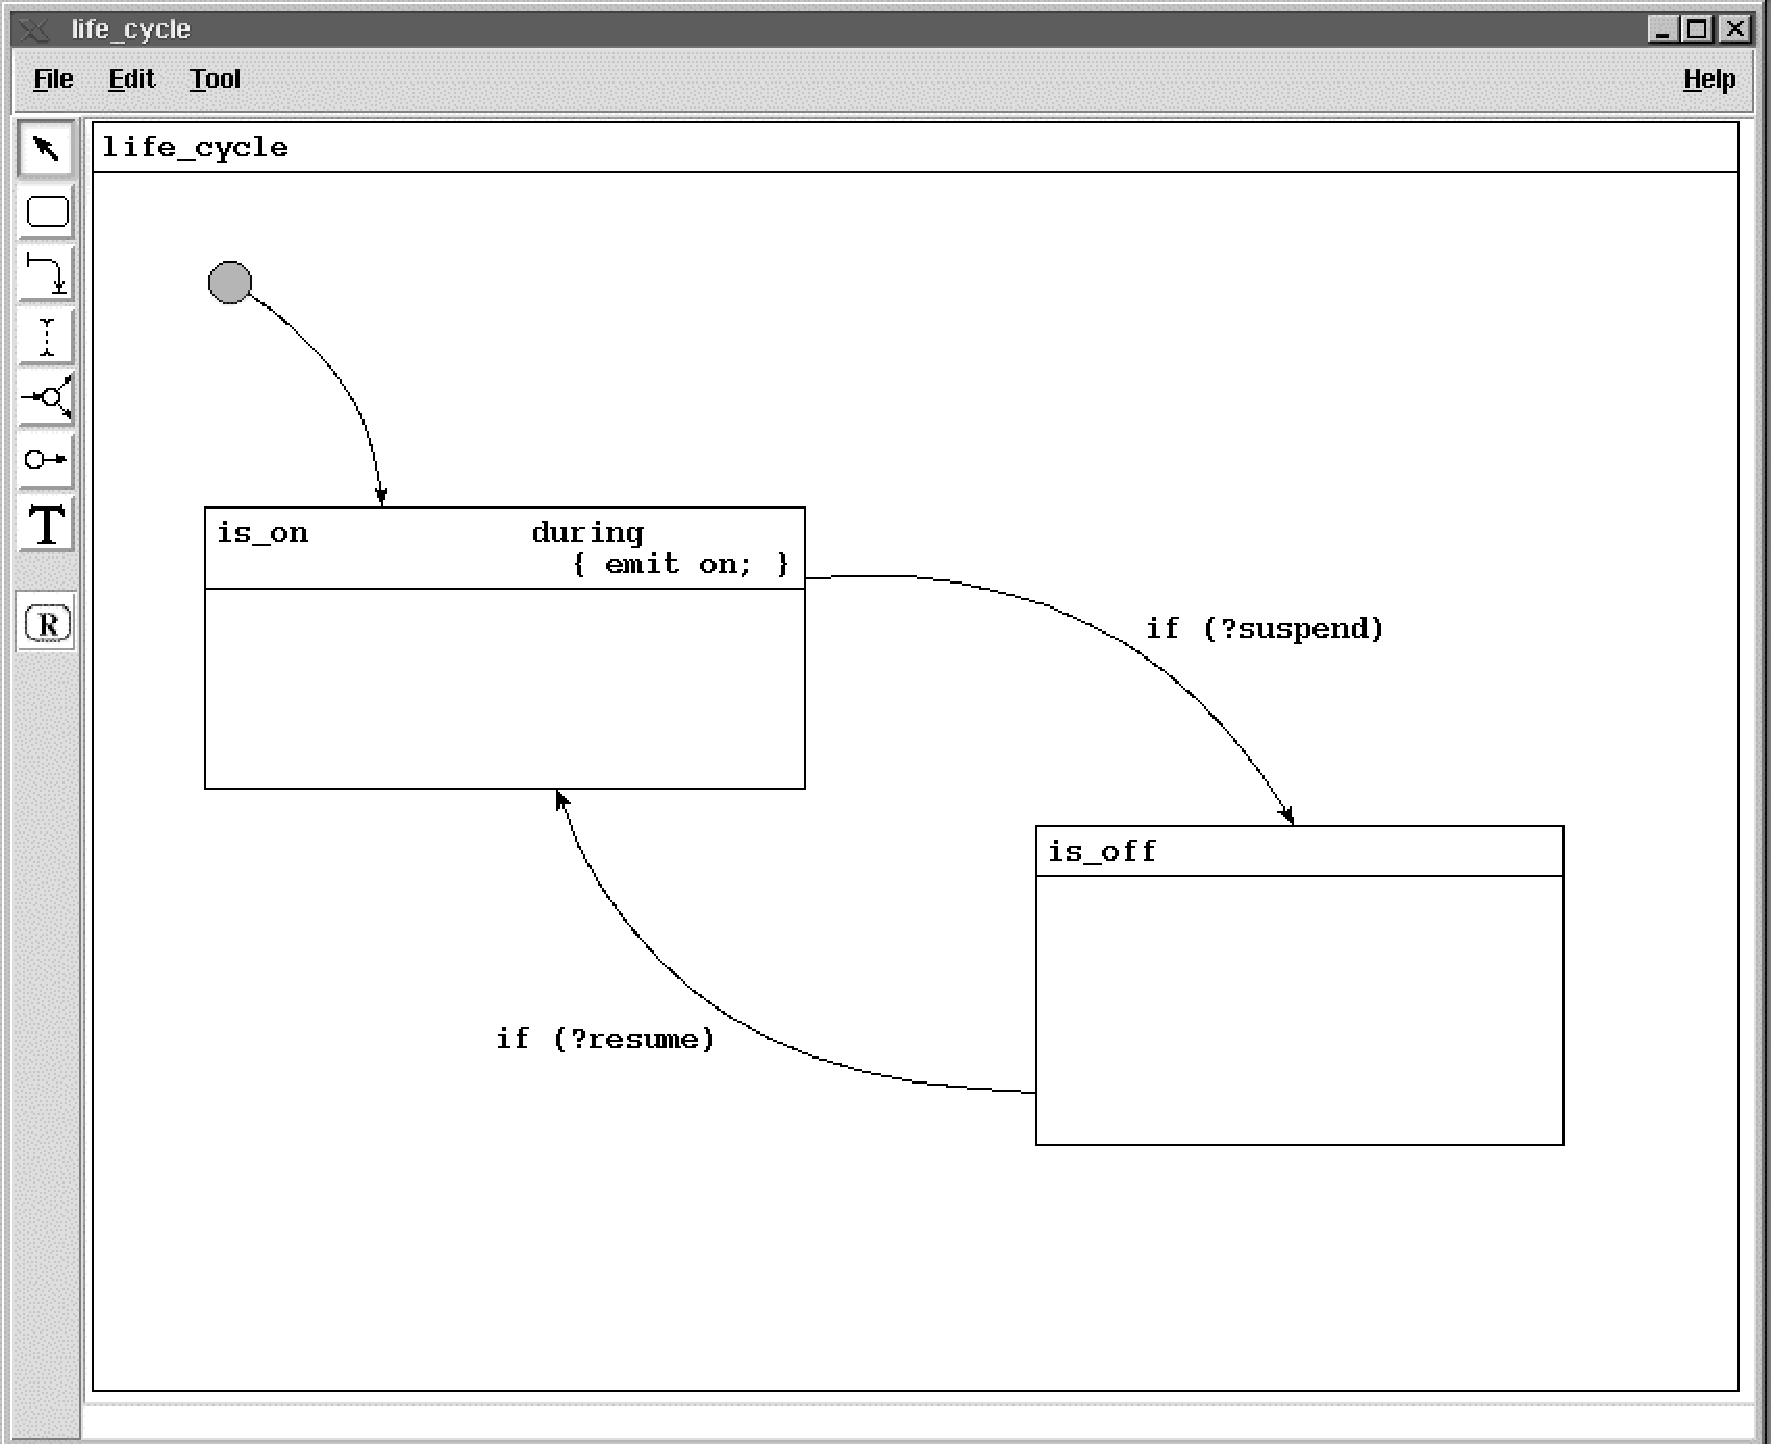
\epsfig{file=rctsty.epsf,width=300pt}
% \end{center}
% 
% 
% \paragraph{Blackboard implementation.} Blackboards are programmed in C and
% have to be started before any synchronous process may register.  In
% the present implementation, blackboards are based on the TCP/IP
% protocol.
% 
% If a synchronous process is created it automatically registers with
% blackboards (and automatically de-registers if terminated). Several
% synchronous processes may register at the same blackboard.
% 
% The protocol is thus: emittance of a network signal is transmitted to
% the blackboard at the end of an instant.  The blackboard uses the
% \pp{select then} operation to choose a value if several transmissions
% happen ``at the same time''.  The blackboard transmits the latched
% value to all registered synchronous process.  At each instant, a
% synchronous process polls for the network signals, and applies a memory copy
% to latch the value internally providing it with a time stamp. There
% may be several memory copies if the blackboard is related to several
% input signals.
% 
% This protocol is non blocking in that transmission, polling, and
% memory copy ask for a very small amount of time only (which
% nevertheless has to be considered if minimal cycle times for a
% synchronous process are computed).
